\section{现阶段研究基础}
\begin{frame}{\insertsection——野外取样}
	\begin{center}
		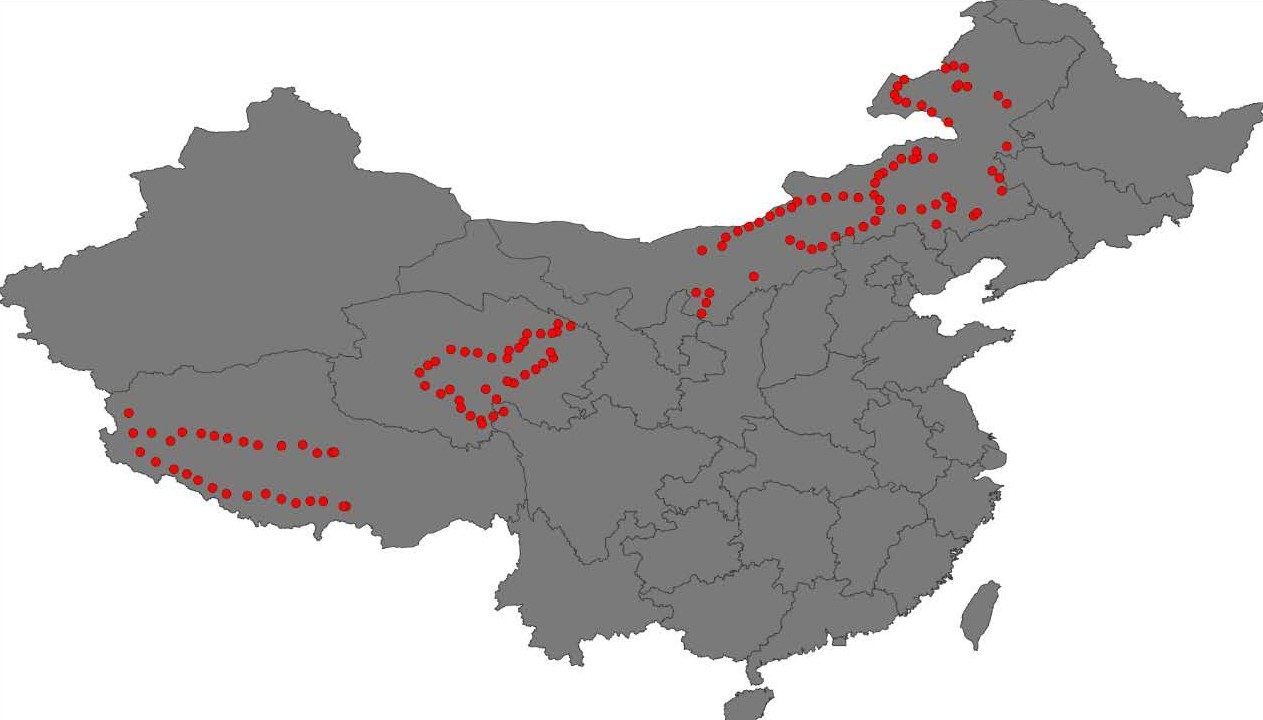
\includegraphics[width = 0.9\textwidth]{./pic/3.1.jpg}
	\end{center}
	126个样点
	\begin{itemize}
		\item 2014-8	西藏:28个样点, 青海:33个样点
		\item 2015-9	内蒙古:65样点
	\end{itemize}
\end{frame}

\subsection{植物样品}
\begin{frame}{\insertsection——植物样品}
		\begin{center}
			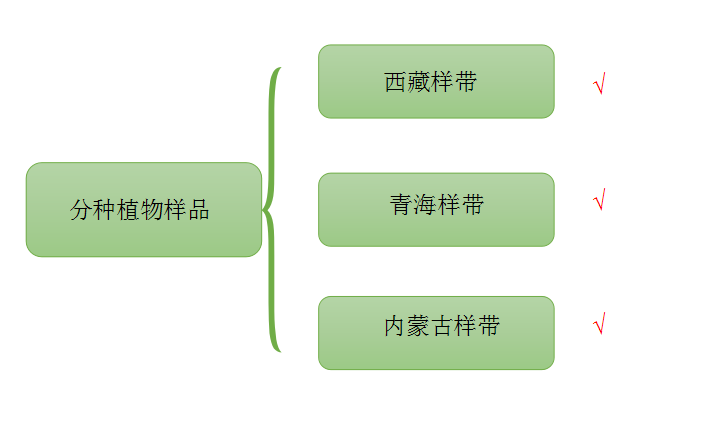
\includegraphics[width = \textwidth]{./pic/3.2.png}
		\end{center}
\end{frame}
\subsection{冷冻土壤样品}
\begin{frame}{\insertsection——冷冻土壤样品}
	\begin{center}
		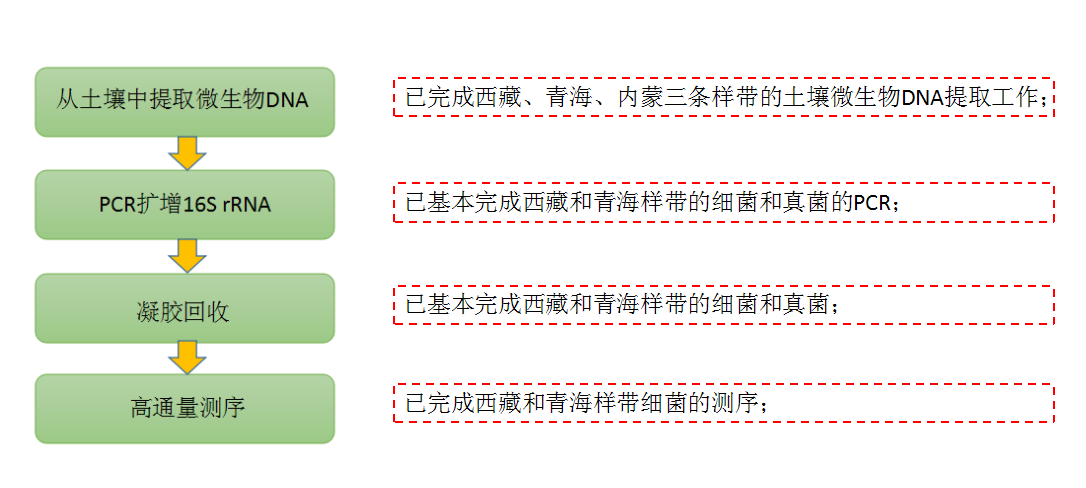
\includegraphics[width = \textwidth]{./pic/3.3.png}
	\end{center}
\end{frame}
\subsection{风干土壤样品}
\begin{frame}{\insertsection——风干土壤样品}
		\begin{center}
			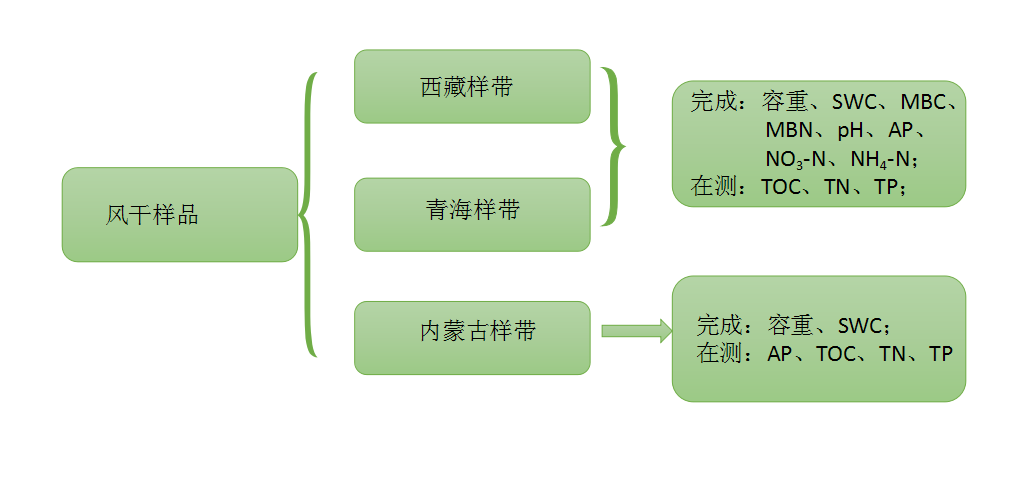
\includegraphics[width = \textwidth]{./pic/3.4.png}
		\end{center}
\end{frame}
